\section{Automatic Stream Management Using Program Contexts}

In developing \textsf{\small PCStream}, our key insight was that in most applications,
(regardless of their I/O workload characteristics)
a few dominant I/O activities exist
and each dominant I/O activity   
represents the application's important I/O context (e.g., for logging or for flushing). 
Furthermore, most dominant I/O activities tend to have distinct data lifetime patterns.
In order to distinguish data by their lifetimes, therefore, 
it is important to effectively distinguish dominant I/O activities from each other.  
For example, in update workloads, 
LBAs alone were effective in separating dominant I/O activities.  

In this paper, we argue that a program context is an efficient general-purpose
indicator for separating dominant I/O activities regardless of the type of I/O
workloads.  Since a PC represents an execution path of an application which
invokes write-related system functions such as {\tt write()} and {\tt writev()}
in the Linux kernel,  we represent the PC by summing program counter values of
all the functions along the execution path which leads to a write system call.
In RocksDB, for example, dominant I/O activities include logging, flushing and
compaction.  Since they are invoked through different function-call paths, we
can easily identify dominant I/O activities of RocksDB using PCs.  For example,
Fig.~\ref{fig:getpc}(a) shows an execution path for flushing in RocksDB.  The
sum of program counter values of \texttt{Run()}, \texttt{WriteLevel0Table()},
and \texttt{BuildTable()} is used to represent the PC for the flushing
activity. Note that using the program context to distinguish data lifetimes is
not new. For example, Ha {\it et al.} proposed a data separation technique
based on the program context~\cite{PCHa}.  However, their work was neither
designed for append-only workloads nor for modern multi-streamed SSDs.

\begin{figure}[t]
\centering
\hfill
%\vspace{-10pt}
	\subfloat[Logging (PC)]{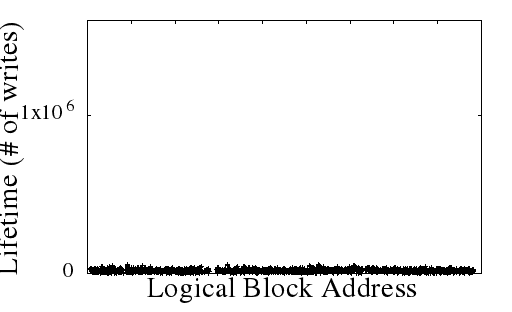
\includegraphics[width=0.2\textwidth]{figure/type_1}} % data from 4/03031953 
	\hspace{2pt}
	\subfloat[Logging (manual)]{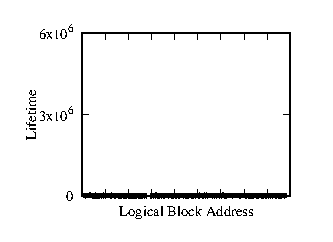
\includegraphics[width=0.2\textwidth]{figure/pcID_2}}
\hfill
\vspace{7pt}
	\subfloat[Flushing (PC)] {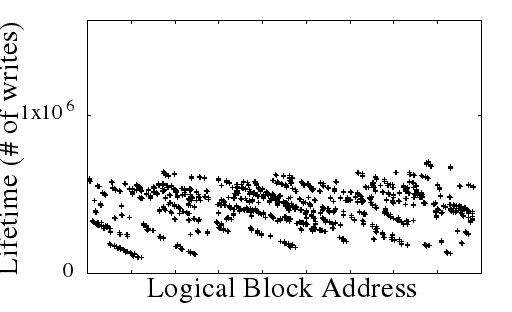
\includegraphics[width=0.2\textwidth]{figure/type_3}}
	\hspace{2pt}
	\subfloat[Flushing (manual)]{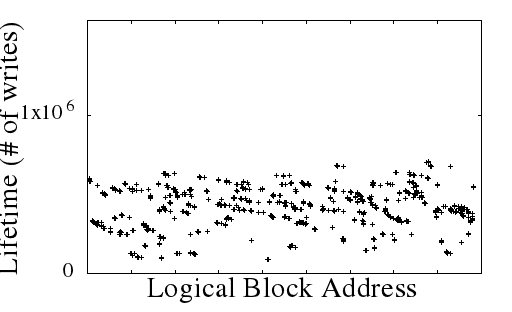
\includegraphics[width=0.2\textwidth]{figure/pcID_3}}
%\vspace{-7pt}
\caption{Data lifetime distributions of different PCs for an append-only workload.} 
\label{fig:types_and_PCs}
%\vspace{-20pt}
\end{figure}

In order to validate our hypothesis that PCs can be useful for predicting
lifetimes by distinguishing dominant I/O activities, we conducted experiments
using RocksDB, comparing the accuracy of identifying dominant I/O activities
using two different methods.  First, we manually identified dominant I/O
activities by inspecting the source code. Second, we automatically decided
dominant I/O activities by extracting PCs for write-related system functions.
Fig.~\ref{fig:types_and_PCs} illustrates two dominant I/O activities matched
between two methods.   As shown in Fig.~\ref{fig:types_and_PCs}(a)
and~\ref{fig:types_and_PCs}(b), the logging activity of RocksDB is correctly
identified by two methods.  Furthermore, from the logging-activity PC, we can
clearly observe that data written from the PC are short-lived. Similarly,
from Fig.~\ref{fig:types_and_PCs}(c) and~\ref{fig:types_and_PCs}(d), we observe
that data written from the flushing-activity PC behave in a different fashion.
For example, data from the flushing-activity PC remain valid a lot longer than
those from the logging-activity PC.

Furthermore, PCs are also effective for non-append-only workloads
in distinguishing I/O activities. 
In order to show the effect of PCperformed experiments 

\begin{figure}[t]
\centering
\hfill
%\vspace{-10pt}
	\subfloat[sqlite (PC)]{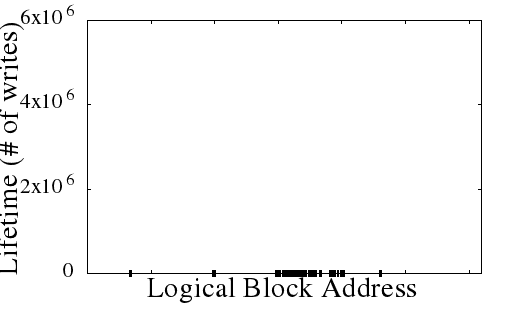
\includegraphics[width=0.2\textwidth]{figure/sqlite_short_LBA}} % data from py-tpcc/4/09151534
	\hspace{2pt}
	\subfloat[sqlite (manual)]{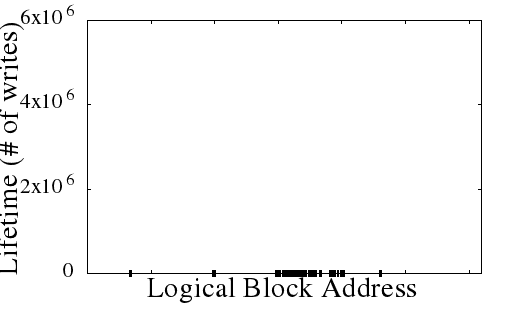
\includegraphics[width=0.2\textwidth]{figure/sqlite_short_LBA_manual}}
\hfill
\vspace{7pt}
	\subfloat[gcc (PC)] {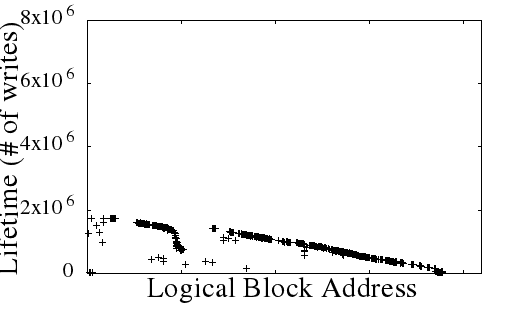
\includegraphics[width=0.2\textwidth]{figure/compile_short_PC}}
	\hspace{2pt}
	\subfloat[gcc (manual)]{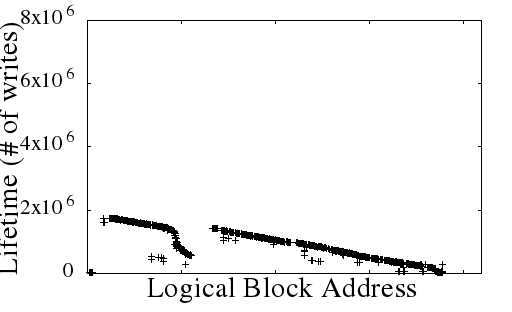
\includegraphics[width=0.2\textwidth]{figure/compile_short_manual}}
%\vspace{-7pt}
\caption{Data lifetime distributions of different PCs for updating workloads.} 
\label{fig:types_and_PCs}
%\vspace{-20pt}
\end{figure}


